%! suppress = TooLargeSection
%! Author = aybehrouz
%! Date = 2/28/21


\documentclass[11pt, a4paper]{report}
\usepackage[a4paper]{geometry}

% Packages
\usepackage{tipa}
\usepackage{graphicx}
\usepackage{hyperref}
\usepackage{amsfonts}
\usepackage[ruled,boxed]{algorithm2e}
\usepackage{algpseudocode}
\usepackage{listings}
\usepackage{amssymb}
\usepackage{tcolorbox}
\usepackage{amsmath}



%\binoppenalty=99999
%\relpenalty=99999
\newcommand{\note}[1] {
    \begin{tcolorbox}[colframe=white,colback=white]
        \emph{#1}
        %\emph{#1}\medskip
    \end{tcolorbox}
}

\title{Argennon: A Scalable Smart Contract Platform}
\author{aybehrouz}
\date{January 2021}


\begin{document}
    %\maketitle
    \tableofcontents


    \chapter{The Argennon Smart Contract Execution Environment}\label{ch:AVM}
    %! Author = aybehrouz
%! Date = 2/28/21

% Preamble
\documentclass[11pt, A4]{report}

% Packages
%\usepackage{amsmath}
\usepackage{graphicx}
\graphicspath{ {../img/} }
\usepackage{hyperref}
\usepackage{amsfonts}
\usepackage[ruled,boxed]{algorithm2e}
\usepackage{algpseudocode}
\usepackage{listings}
\usepackage{amssymb}
\lstset{
%  basicstyle=\ttfamily,
    mathescape
}
%\binoppenalty=99999
%\relpenalty=99999

\title{The Argennon Virtual Machine}
\author{aybehrouz}
\date{January 2021}

% Document
\begin{document}
    \maketitle


    \chapter{Specification}\label{ch:specification}


    \section{Introduction}\label{sec:introduction}

    The Argennon Virtual Machine (AVM) is an abstract computing machine for executing Argennon's smart contracts. It
    is designed in a way that it could be efficiently implemented in either hardware or software.


    \section{The Structure of the Argennon Virtual Machine}\label{sec:the-structure-of-the-algorand-virtual-machine}

    ...

    \subsection{Data Types}\label{subsec:data-types}

    The Argennon Virtual Machine expects that all type checking is done prior to run time, typically by a compiler,
    and does not have to be done by the Argennon Virtual Machine itself.

    The instruction set of the Argennon Virtual Machine distinguishes its operand types using instructions intended to
    operate on values of specific types. For instance, \texttt{iadd} assumes that its operands are two 64-bit integers.

    \subsection{The \texttt{PC} Register}\label{subsec:the-pc-register}

    ...

    \subsection{Call Stack}\label{subsec:call-stack}

    A call stack contains the information that is needed for restoring the state of the invoker of a method.

    \subsection{Memory Unit}\label{subsec:memory-unit}

    The Argennon Virtual Machine has a byte addressable memory which is divided into separate segments. Every segment
    belongs to a smart contract that has a unique \texttt{applicationID}. The AVM always has a single working memory
    segment and memory locations outside its current working segment can not be accessed. The only instructions which
    can change the current working segment are \texttt{invoke\_external}, \texttt{athrow} and return instructions.

    Every smart contract has its own memory segment. Hence, there is no way for a smart contract to access another
    smart contract's memory. Interaction between smart contracts is done using \texttt{invoke\_external} instruction,
    and a smart contract can invoke methods of another smart contract by this instruction.

    A memory segment consists of five data areas:
    \begin{itemize}
        \item Code Area
        \item Constant Area
        \item Local Frame
        \item Operand Stack
        \item Heap
    \end{itemize}
    All data areas except operand stack, have their own address space which starts from 0. Operand stack is a
    last-in-first-out (LIFO) stack and is not addressable. Every memory access instruction operates on its specific
    data areas.

    \subsubsection{Code Area}

    The code area of a segment contains the byte-code of the smart contract which owns that segment. The AVM has no
    instructions for manipulating the code area. \textbf{Installing, removing and updating smart contracts need to
    be done externally.}

    \subsubsection{Constant Area}

    The constant area of a segment contains several kinds of constants, ranging from user defined constants to method
    address tables. A method address table stores method locations in the code area and their access type. The access
    type of a method can be either \texttt{public} or \texttt{private}. The AVM has no instructions for modifying the
    constant area.

    \emph{Only public methods can be invoked by \texttt{invoke\_external} instruction.}

    \subsubsection{Local Frame}

    A local frame is used to store methods parameters and local variables. A new frame is created each time a method
    is invoked, and it is destroyed when its method invocation completes, whether the completion is normal or abrupt.

    \subsubsection{Operand Stack}

    Every time a local frame is created, a corresponding empty last-in-first-out (LIFO) stack is created too. AVM
    instructions take operands from the operand stack, operate on them, and push the result back onto the operand
    stack. An operand stack is destroyed when its owner method completes, whether that completion is normal or abrupt.

    \subsubsection{Heap}

    The heap of a segment is a persistent memory area which is divided into pages. Memory locations inside every page
    have a separate address space that starts from 0, and each page can be referenced by an index that starts from 0. In
    other words, the address of every memory location inside a heap is a pair of indices: \texttt{(pageIndex, offset)}.
    Different pages of a heap do not need to be equally sized.

    \emph{The reason behind this paged design is that the heap is usually persisted using a block device. A heap with
    a paged structure could expose the underlying block based nature of the persistence layer to the application
    layer. In this way, the compiler or the programmer could better optimize the code for the persistence layer.}


    \section{Instruction Set Summary}\label{sec:instruction-set-summary}

    An Argennon Virtual Machine instruction consists of a \textbf{one-byte} opcode specifying the operation to be
    performed, followed by zero or more operands supplying arguments or data that are used by the operation.
    \textbf{The number and size of the operands are determined solely by the opcode.}

    \subsection{Method Invocation}\label{subsec:method-invocation}

    The Argennon Virtual Machine has three types of method invocation:
    \begin{itemize}
        \item \texttt{invoke\_internal} invokes a method from the current running smart contract.
        \item \texttt{invoke\_external} invokes a \texttt{public} method from another smart contract. It will change
        the current memory segment to the segment of the invoked smart contract.
        \item \texttt{invoke\_native} invokes a method that is not hosted by the Argennon virtual machine. By this
        instruction, high performance native methods of the hosting machine could become available to AVM smart
        contracts.
    \end{itemize}

    \emph{In the future, we may need to add special instructions for invoking interface and virtual methods...}

    Each time a method is invoked a new local frame and operand stack is created. The Argennon Virtual Machine uses
    local frames to pass parameters on method invocation. On method invocation, any parameters are passed in
    consecutive local variables stored in the method's local frame starting from local variable 0. The invoker of a
    method writes the parameters in the local frame of the invoked method using \texttt{arg} instructions.

    \subsubsection{Exceptions}

    An exception is thrown programmatically using the \texttt{athrow} instruction. Exceptions can also be thrown by
    various Argennon Virtual Machine instructions if they detect an abnormal condition. Some exceptions are not
    catchable and will always abort the execution of the smart contract.

    \subsubsection{Method Invocation Completion}

    A method invocation completes normally if that invocation does not cause an exception to be thrown, either
    directly from the AVM or as a result of executing an explicit throw statement. If the invocation of the current
    method completes normally, then a value may be returned to the invoking method. This occurs when the invoked
    method executes one of the return instructions, the choice of which must be appropriate for the type of the value
    being returned (if any). Execution then continues normally in the invoking method's local frame with the returned
    value (if any) pushed onto the operand stack.

    A method invocation completes abruptly if an exceptions is thrown and is not caught by the current method. A
    method invocation that completes abruptly never returns a value to its invoker.

    When a method completes, whether normally or abruptly, the call stack is used to restore the state of the invoker,
    including its local frame and operand stack, with the \texttt{PC} register appropriately restored and incremented
    to skip past the method invocation instruction. If the invoker was another smart contract, i.e.\ the invocation
    was made by an \texttt{invoke\_external} instruction, the current memory segment will be changed to the invoker's
    segment.

    A thrown exception causes methods in the call stack to complete \textbf{abruptly} one by one, as long as the
    \texttt{PC} register is not pointing to a \texttt{catch} instruction. The \texttt{catch} instruction acts like a
    branch instruction that branches only if an exception is caught. \textbf{When an external method invocation
    completes abruptly, before changing the current segment, all changes made to the heap area by that method
    call, including changes made to other segments, will be rolled back.} So, when a method call completes abruptly,
    that method call essentially has no effect on the AVM state.

    \emph{By using the \texttt{athrow} instruction properly, a programmer can make any method act like an atomic
    operation.}

    \subsection{Authorizing Operations}\label{subsec:authorizing-operations}

    In blockchain applications, we usually need to authorize certain operations. For example, for sending an asset
    from a user to another user, first we need to make sure that the sender has authorized this operation. The
    Argennon virtual machine has no built in mechanism for authorizing operations, but it provides a rich set of
    cryptographic instructions for validating signatures and cryptographic entities. By using these instructions and
    passing signatures as parameters to methods, a programmer can implement the required logic for authorizing any
    operation.

    \emph{The Argennon virtual machine has no instructions for issuing cryptographic signatures.}

    In addition to signatures, a method can verify its invoker by using \texttt{get\_parent} instruction. This
    instruction gets the \texttt{applicationID} of the smart contract that is one level deeper than the current
    smart contract in the call stack. In other words, it returns the \texttt{applicationID} of the smart contract that
    has invoked the current smart contract. (if any)

    \subsection{Heap Allocation Instructions}\label{subsec:heap-allocation-instructions}

    ...


    \section{The AVM Standard Library}\label{sec:the-avm-standard-library}

    ...


    \chapter{Implementation}\label{ch:implementation}


    \section{Persistence}\label{sec:persistence}

    For implementing the persistence layer of the AVM, we assume that we have access to an updatable zero-knowledge
    elementary database (ZK-EDB) with the following properties:

    \begin{itemize}
        \item The ZK-EDB contains a mapping from a set of keys to a set of values.
        \item Every state of the database has a commitment \(C\).
        \item The ZK-EDB has a method \((D, p) = get(x)\), where \(x\) is a key and \(D\) is the associated data
        with \(x\), and \(p\) is a proof.
        \item A user can use \(C\) and \(p\) to verify that \(D\) is really associated with \(x\), and \(D\) is not
        altered. Consequently, a user who can obtain \(C\) from a trusted source does not need to trust the ZK-EDB.
        \item Having \(p\) and \(C\) a user can compute the commitment \(C'\) for the database in which \(D'\) is
        associated with \(x\) instead of \(D\).
    \end{itemize}

    We use a ZK-EDB for storing the AVM heap. We include the commitment of the current state of this DB in every
    block of the Argennon blockchain, so ZK-EDB servers need not be trusted servers.

    Every page of AVM heap will be stored with a key of the form: \texttt{applicationID|pageIndex} (the \texttt{|}
    operator concatenates two numbers). Nodes do not keep a full copy of the AVM heap and for validating block
    certificates or emulating the AVM ( i.e.~validating transactions) they need to connect to a ZK-EDB and retrieve
    the required pages of AVM heap. For better performance, nodes keep a cache of heap pages to
    reduce the amount of ZK-EDB access.

    We also use a ZK-EDB for storing the code area of each segment, and we include the commitment of this DB in every
    block. Every code area will be divided into blocks and every block will be stored in the DB with
    \texttt{applicationID|blockID} as its key. Like heap pages, nodes keep a cache of code area blocks.

    \emph{Unlike heap pages, the AVM is not aware of different blocks of code area.}


    \section{Transactions}\label{sec:transactions}

    Argennon has four types of transaction:

    \begin{itemize}
        \item \texttt{avmCall} essentially is an \texttt{invoke\_external} instruction that invokes a method from an
        AVM smart contract. Users interact with AVM smart contracts using these transactions. Transferring all
        assets, including ARGs, is done by these transactions.
        \item \texttt{installApp} installs an AVM smart contract and determines the update policy of the smart
        contract: if the contract is updatable or not, which accounts can update or uninstall the contract, and so
        on.
        \item \texttt{unInstallApp} removes an AVM smart contract.
        \item \texttt{updateApp} updates an AVM smart contract.
    \end{itemize}

    All types of Argennon transactions contain an \texttt{invoke\_external} instruction which calls a special method
    from ARG smart contract that transfers the proposed fee of the transaction in ARGs from a sender account to the
    fee sink accounts.

    Every transaction is required to exactly specify what heap locations or code area addresses it will access. This
    enables validators to start retrieving the required memory blocks from available ZK-EDB servers as soon as they
    see a transaction, and they won't need to wait for receiving the new proposed block. A transaction that tries to
    access a memory location that is not included in its access lists, will be rejected. Users could use smart contract
    oracles to predict the list of memory blocks their transactions need. See Section~\ref{sec:smart-contract-oracle}
    for more details.


    \section{Blockchain}\label{sec:blockchain}

    Every block of the Argennon blockchain corresponds to a set of transactions. We store the commitment of this
    transaction set in every block, but we don't keep the set itself. To be able to detect replay attacks, we require
    every signature that a user creates to have a nonce. This nonce consists of the issuance round of the signature
    and a sequence number: \texttt{(issuance,\ sequence)}. When a user creates more than one signature in a round, he
    must sequence his signatures starting from 0 (i.e.~the sequence number restarts from 0 in every round). We define
    a maximum lifetime for signatures, so a signature is invalid if \texttt{currentRound - issuance \textgreater{}\
        maxLifeTime} or if a signature of the same user with a bigger or equal nonce is already used
    (i.e.~is recorded in the blockchain). A nonce is bigger than another nonce if it has an older issuance. If two
    nonces have an equal issuance, the nonce with the bigger sequence number will be considered bigger.

    To be able to detect invalid signatures, we keep the maximum nonce of used digital signatures per user. When the
    difference between \texttt{issuance} component of this nonce and the current round becomes bigger than the
    maximum allowed lifetime of a signature, this information can be safely deleted. \textbf{As a result, we will not
    have the problem of "un-removable empty accounts" like Ethereum.}

    The only information that Argennon nodes are required to store is \textbf{the most recent block} of the Argennon
    blockchain. Every block of the Argennon blockchain contains the following information:

    \begin{center}
        \begin{tabular}{||c||}
            \hline
            Block \\ [0.5ex]
            \hline\hline
            commitment to the ZK-EDB storing heap pages \\ [0.7ex]
            commitment to the ZK-EDB storing code areas \\ [0.7ex]
            commitment to the set of transactions       \\ [0.7ex]
            previous block hash                         \\ [0.7ex]
            random seed                                 \\ [0.7ex]
            \hline
        \end{tabular}
    \end{center}

    For confirming a new block, nodes that are not validators only need to verify the block certificate. For
    verifying a block certificate, a node needs to know the ARG balances of validators, but it doesn't need to
    emulate the AVM execution.

    On the other hand, nodes that are chosen to be validators, for validating a new block, need to emulate the
    execution of the Argennon virtual machine. To do so, first they retrieve all heap pages and code area blocks they
    need from available ZK-EDBs. Then, they emulate the execution of AVM instructions and validate all the
    transactions included in the new block. This will modify some pages of the AVM memory, so they update the ZK-EDB
    commitments based on the modified pages and verify the commitments included in the new block. Validators also
    calculate and verify the commitment to the new block's transaction set.

    \emph{Validators do not need to write the modified pages back to ZK-EDB servers. ZK-EDBs will receive the new
    block, and they will update their database by emulating the AVM execution.}


    \section{Incentive mechanism}\label{sec:incentive-mechanism}

    \subsection{Transaction Fee}\label{subsec:transaction-fee}

    Every transaction in the Argennon blockchain starts with an \texttt{invoke\_external} instruction which calls a
    special method from ARG smart contract. This method will transfer the proposed fee of the transaction in ARGs
    from a sender account to the fee sink accounts. Argennon has two fee sink accounts: \texttt{execFeeSink} collects
    execution fees and \texttt{dbFeeSink} collects fees for ZK-EDBs. The Protocol decides how to distribute the
    transaction fee between these two fee sink accounts.

    When a block is added to the blockchain, the proposer of that block will receive a share of the block fees.
    Consequently, a block proposer is always incentivized to include more transactions in his block. However, if he
    puts too many transactions in his block and the validation of the block becomes too difficult, some validators
    may not be able to validate all transactions on time. If a validator can not validate a block in the required
    time, he will consider the block invalid. So, when a proposed block contains too many transactions, the network
    may reach consensus on another block, and the proposer of that block will not receive any fees. As a result, a
    proposer is incentivized to use network transaction capacity optimally.

    On the other hand, we believe that the proposer does not have enough incentives for optimizing the storage size
    of the transaction set. Therefore, we require that \textbf{the size of the transaction set of every block in
    bytes be lower than a certain threshold.}

    Validators need to spend resources for validating transactions. When a validator starts the emulation of the AVM
    to validate a transaction, solely from the code he can't predict the time the execution will finish. This will
    give an adversary an opportunity to attack the network by broadcasting transactions that never ends. Since,
    validators can not finish the execution of these transactions, the network will not be able to charge the
    attacker any fees, and he would be able to waste validators resources for free.

    To mitigate this problem, we require that every transaction specify a cap for all the resources it needs. This
    will include memory, network and processor related resources. Also, the protocol defines an execution cost for
    every AVM instruction reflecting the amount of resources its emulation needs. This will define a standard way for
    measuring the execution cost of any \texttt{avmCall} transaction. Every \texttt{avmCall} transaction is required
    to specify a maximum execution cost. If during emulation it reaches this maximum cost, the transaction will be
    considered failed and the network can receive the proposed fee of that transaction.

    Every \texttt{avmCall} transaction is required to provide the following information as an upper bound for the
    resources it needs:

    \begin{itemize}
        \item Execution cost
        \item A list of heap/code-area locations for reading
        \item A list of heap locations for writing
        \item A list of heap pages it will deallocate
        \item Number and size of heap pages it will allocate
    \end{itemize}

    If a transaction tries to violate any of these predefined limitations, for example, if it tries to read a memory
    location that is not included in its reading list, it will be considered failed and the network can receive the
    proposed fee of that transaction.

    \emph{A transaction always pays all of its proposed fee, no matter how much of its predefined resources were not
    used in the final emulation.}

    \subsection{ZK-EDB Servers}\label{subsec:zk-edb-servers}

    The incentive mechanism for ZK-EDB servers should have the following properties:

    \begin{itemize}
        \item It incentivizes storing all memory blocks, whether a heap page or a code area block, and not only those
        which are used more frequently.
        \item It incentivizes ZK-EDB servers to actively provide the required memory blocks for validators.
        \item Making more accounts will not provide any advantages for a ZK-EDB server.
    \end{itemize}

    For our incentive mechanism, we require that every time a validator receives a memory block from a ZK-EDB, after
    validating the data, he give a receipt to the ZK-EDB. In this receipt the validator signs the following information:

    \begin{itemize}
        \item \texttt{ownerAddr}: the ARG address of the ZK-EDB\@.
        \item \texttt{receivedBlockID}: the ID of the received memory block.
        \item \texttt{round}: the current round number.
    \end{itemize}

    \emph{In a round, an honest validator never gives a receipt for an identical memory block to two different ZK-EDBs.}

    To incentivize ZK-EDB servers, a lottery will be held every round and a predefined amount of ARGs from
    \texttt{dbFeeSink} account will be distributed between winners as a prize. This prize will be divided equally
    between all \emph{winning tickets} of the lottery.

    \emph{One ZK-EDB server could own multiple winning tickets in a round.}

    To run this lottery, every round, based on the current block seed, a collection of \emph{valid} receipts will be
    selected randomly as the \emph{winning receipts} of the round. A receipt is \emph{valid} in the round \(r\) if:

    \begin{itemize}
        \item The signer was a validator in the round \(r - 1\) and voted for the agreed-upon block.
        \item The data block in the receipt was needed for validating the \textbf{previous} block.
        \item The receipt round number is \(r - 1\).
        \item The signer did not sign a receipt for the same data block for two different ZK-EDBs in the previous round.
    \end{itemize}
    For selecting the winning receipts we could use a random generator:
    \begin{verbatim}
IF random(seed|validatorPK|receivedBlockID) < winProbability THEN
    the receipt issued by validatorPK for receivedBlockID is a winner
    \end{verbatim}
    \begin{itemize}
        \item \texttt{random()} produces uniform random numbers between 0 and 1, using its input argument as a seed.
        \item \texttt{validatorPK} is the public key of the signer of the receipt.
        \item \texttt{receivedBlockID} is the ID of the memory block that the receipt was issued for.
        \item \texttt{winProbability} is the probability of winning in every round.
        \item \texttt{seed} is the current block seed.
        \item \texttt{|} is a concatenation operator.
    \end{itemize}

    \emph{The winners of the lottery were validators one round before the lottery round.}

    Also, based on the current block seed, a random memory block, whether a heap page or a code area block, is
    selected as the challenge of the round. A ZK-EDB that owns a winning receipt needs to broadcast a \emph{winning
    ticket} to claim his prize. The winning ticket consists of a winning receipt and a \emph{solution} to the round
    challenge. Solving a round challenge requires the content of the memory block which was selected as the round
    challenge. This will encourage ZK-EDBs to store all memory blocks.

    A possible choice for the challenge solution could be the cryptographic hash of the content of the challenge
    memory block combined with the ZK-EDB ARG address: \texttt{hash(challenge.content|ownerAddr)}

    The winning tickets of the lottery of the round \(r\) need to be included in the block of the round \(r\),
    otherwise they will be considered expired. Validation and prize distribution for the winning tickets of the round
    \(r\) will be done in the round \(r + 1\). This way, \textbf{the content of the challenge memory block could be
    kept secret during the lottery round.} Every winning ticket will get an equal share of the lottery prize.

    \subsection{Memory Allocation and De-allocation}\label{subsec:memory-allocation-and-de-allocation}

    Every \(k\) round the protocol chooses a price per byte for AVM memory. When a smart contract executes a heap
    allocation instruction, the protocol will automatically deduce the cost of the allocated memory from the ARG
    address of the smart contract.

    To determine the price of AVM memory, Every \(k\) round, the protocol calculates \texttt{dbFee} and
    \texttt{memTraffic} values. \texttt{dbFee} is the aggregate amount of collected database fees, and
    \texttt{memTraffic} is the total memory traffic of the system. For calculating the memory traffic of the system
    the protocol considers the total size of all the memory pages that were accessed for either reading or writing
    during a time period. These two values will be calculated for the last \(k\) rounds and the price per byte of
    AVM memory will be a linear function of \texttt{dbFee/memTraffic}

    When a smart contract executes a heap de-allocation instruction, the protocol will refund the cost of
    de-allocated memory to the smart contract. Here, the current price of AVM memory does not matter and the protocol
    calculates the refunded amount based on the average price the smart contract had paid for that allocated memory.
    This will prevent smart contracts from profit taking by trading memory with the protocol.


    \section{Concurrency}\label{sec:concurrency}

    \subsection{Memory Dependency Graph}\label{subsec:memory-dependency-graph}

    Every block of the Argennon blockchain contains a list of transactions. This list is an ordered list and the
    effect of its contained transactions must be applied to the AVM state sequentially as they appear in the ordered
    list. This ordering is solely chosen by the block proposer, and users should not have any assumption about
    the ordering of transactions in a block.

    The fact that block transactions constitute a sequential list, does not mean they can not be executed and applied
    to the AVM state concurrently. Many transactions are actually independent and the order of their execution does not
    matter. These transactions can be safely validated in parallel by validators.

    A transaction can change the AVM state by modifying either the code area or the AVM heap. In Argennon, all
    transactions declare the list of memory locations they want to read or write. This will enable us to determine the
    independent sets of transactions which can be executed in parallel. To do so, we define the \emph{memory dependency
    graph} \(G_d\) as follows:

    \begin{itemize}
        \item \(G_d\) is an undirected graph.
        \item Every vertex in \(G_d\) corresponds to a transaction and vice versa.
        \item Vertices \(u\) and \(v\) are adjacent in \(G_d\) if and only if \(u\) has a memory location \(L\) in its
        writing list and \(v\) has \(L\) in either its writing list or reading list.
    \end{itemize}

    If we consider a proper vertex coloring of \(G_d\), every color class will give us an independent set of
    transactions which can be executed concurrently. To achieve the highest parallelization, we need to color \(G_d\)
    with minimum number of colors. The \emph{chromatic number} of the memory dependency graph thus shows how good a
    transaction set could be run concurrently.

    Graph coloring is computationally NP-hard. However, in our use case we don't need to necessarily find an optimal
    solution. An approximate greedy algorithm will perform well enough in most circumstances.

    After constructing the memory dependency graph of a transaction set, we can use it to construct the
    \emph{execution DAG} of transactions. The execution DAG of a transaction set \(T\) is a directed acyclic
    graph \(G_e\) which has the \emph{execution invariance} property:
    \begin{itemize}
        \item Every vertex in \(G_e\) corresponds to a transaction in \(T\) and vice versa.
        \item Applying the transactions of \(T\) in any order that \emph{respects} \(G_e\) will result in
        the same AVM state.
        \begin{itemize}
            \item An ordering of transactions of \(T\) respects \(G_e\) if for every directed edge \((u,v)\) in \(G_e\)
            the transaction \(u\) comes before the transaction \(v\) in the ordering.
        \end{itemize}
    \end{itemize}

    Having the execution DAG of a set of transactions, using Algorithm~\ref{alg:exec_dag}, we can apply the transaction
    set to the AVM state concurrently, using multiple processor, while we can make sure that the resulted AVM state will
    always be the same no matter how many processor we have used.

    %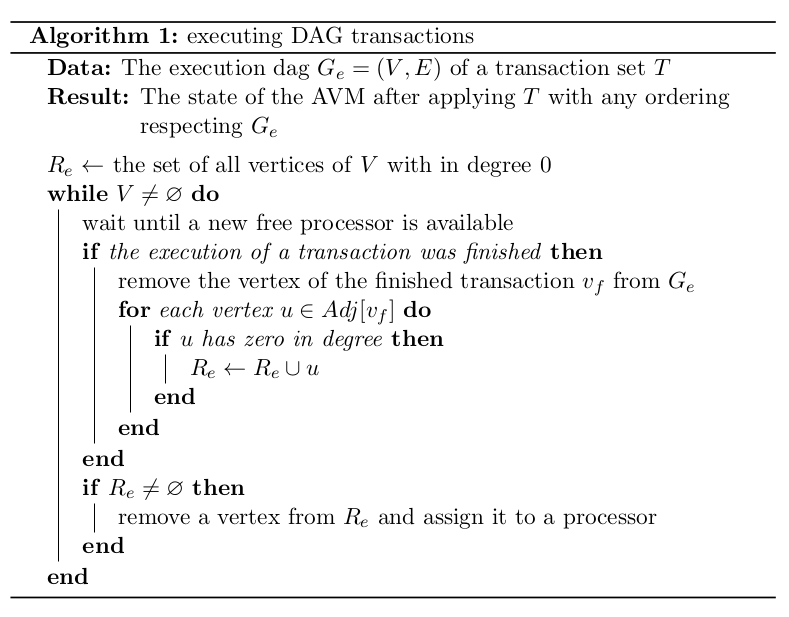
\includegraphics[width=17cm]{../img/Alg1s.png}
    \begin{algorithm}
        \DontPrintSemicolon
        \SetKwData{Ready}{$R_e$}\SetKwData{V}{$v_f$}\SetKwData{Graph}{$G_e$}\SetKwData{Vertices}{$V$}\SetKwData
        {Txns}{$T$}
        \KwData{The execution dag $\Graph = (\Vertices,E)$ of a transaction set \Txns}
        \KwResult{The state of the AVM after applying \Txns with any ordering respecting \Graph}
        \BlankLine
        \Ready $\gets$ the set of all vertices of \Vertices with in degree 0\;
        \While{$\Vertices \neq \varnothing$}
        {
            wait until a new free processor is available\;
            \If{the execution of a transaction was finished}
            {
                remove the vertex of the finished transaction \V from \Graph\;
                \For{each vertex $u \in Adj[\V]$}
                {
                    \If{$u$ has zero in degree}
                    {
                        $\Ready \gets \Ready \cup u$\;
                    }
                }
            }
            \If{$\Ready \neq \varnothing$}
            {
                remove a vertex from \Ready and assign it to a processor\;
            }
        }
        \caption{executing DAG transactions}\label{alg:exec_dag}
    \end{algorithm}

    By replacing every undirected edge of a memory dependency graph with a directed edge in such a way that the
    resulted graph has no cycles, we will obtain a valid execution DAG. Thus, from a memory dependency graph different
    execution DAGs can be constructed with different levels of parallelization ability.

    If we assume that we have unlimited number of processors and all transactions take equal time for executing, it
    can be shown that by providing a minimal graph coloring to Algorithm~\ref{alg:gen_dag} as input, the resulted
    DAG will be optimal, in the sense that it results in the minimum overall execution time.

    %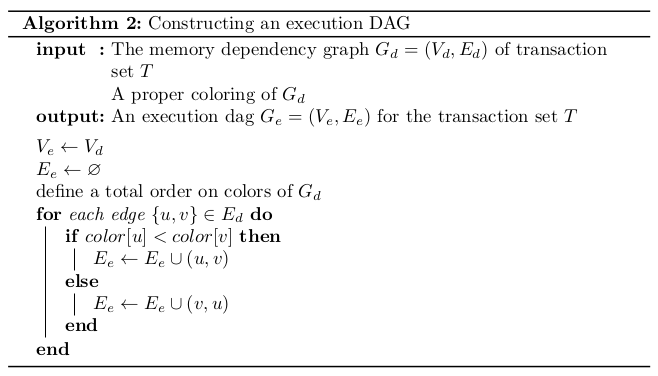
\includegraphics[width=17cm]{../img/Alg2s.png}
    \begin{algorithm}
        \DontPrintSemicolon
        \SetKwData{Txns}{$T$}\SetKwData{Gd}{$G_d=(V_d,E_d)$}
        \SetKwInOut{Input}{input}\SetKwInOut{Output}{output}
        \Input{The memory dependency graph \Gd of a transaction set \Txns\\A proper coloring of $G_d$}
        \Output{An execution dag $G_e=(V_e,E_e)$ for the transaction set \Txns}
        \BlankLine
        $V_e \gets V_d$\;
        $E_e \gets \varnothing$\;
        define a total order on colors of $G_d$\;
        \For{each edge $\{u,v\} \in E_d$}
        {
            \eIf{$color[u] < color[v]$}
            {
                $E_e \gets E_e \cup (u,v)$\;
            }{
                $E_e \gets E_e \cup (v,u)$\;
            }
        }
        \caption{Constructing an execution DAG}\label{alg:gen_dag}
    \end{algorithm}

    The block proposer is responsible for proposing an efficient execution DAG alongside his proposed block which will
    determine the ordering of block transactions and help validators to validate transactions in parallel. Since with
    better parallelization a block can contain more transactions, a proposer is incentivized enough to find a good
    execution DAG for transactions.

    \subsection{Concurrent Counters}\label{subsec:concurrent-counters}

    We know that in Argennon every transaction needs to transfer its proposed fee to the \texttt{feeSink} accounts
    first. This essentially makes every transaction a reader and a writer of the memory locations which store the
    balance record of the \texttt{feeSink} accounts. As a result, all transactions in Argennon will be dependant and
    parallelism will be completely impossible. Actually, any account that is highly active, for example the account
    of an exchange or a payment processor, could become a concurrency bottleneck of the system, making all transactions
    which interact with them dependant.

    This problem can be easily solved by using a concurrent counter (CC) for storing the balance of this type of
    accounts. A concurrent counter is a data structure which improves concurrency by using multiple memory locations for
    storing a single counter. The value of the concurrent counter is equal to the sum of its sub counters and it can
    be incremented or decremented by incrementing/decrementing any of the sub counters. This way, a concurrent
    counter trades concurrency with memory usage.

    A pseudocode for implementing a concurrent counter (CC) which returns an error when the value of the counter
    becomes negative, follows:

    %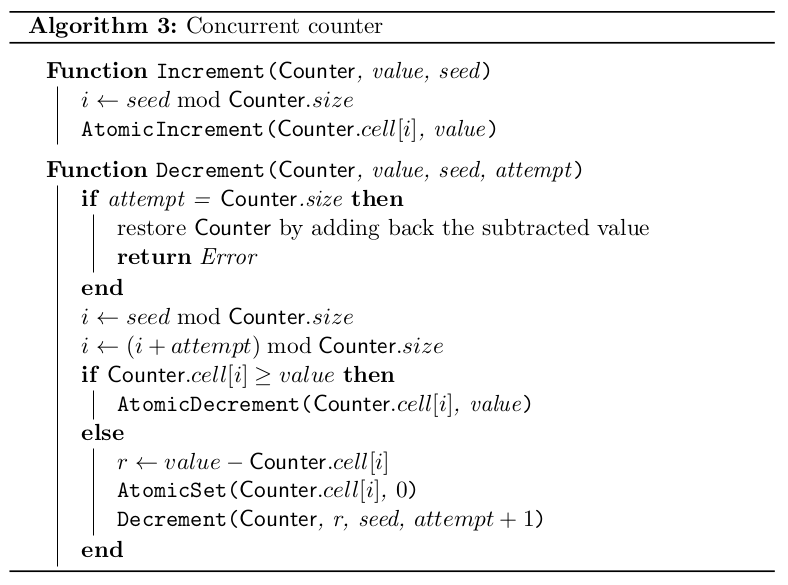
\includegraphics[width=17cm]{../img/Alg3s.png}
    \begin{algorithm}
        \DontPrintSemicolon
        \SetKwData{CC}{Counter}
        \SetKwFunction{Inc}{Increment}\SetKwFunction{Dec}{Decrement}\SetKwFunction{AtomInc}{AtomicIncrement}
        \SetKwFunction{AtomDec}{AtomicDecrement}\SetKwFunction{AtomSet}{AtomicSet}
        \SetKwProg{Fn}{Function}{}{}
        \BlankLine
        \Fn{\Inc{\CC, value, seed}}
        {
            $i \gets seed \bmod \CC.size$\;
           \AtomInc{$\CC.cell[i]$, value}\;
        }
        \BlankLine
        \Fn{\Dec{\CC, value, seed, attempt}}
        {
            \If {attempt = \CC.size}
            {
                restore \CC by adding back the subtracted value\;
                \KwRet{Error}\;
            }
            $i \gets seed \bmod \CC.size$\;
            $i \gets (i + attempt) \bmod \CC.size$\;
            \eIf {$\CC.cell[i] \geq value$}
            {
                \AtomDec{$\CC.cell[i]$, value}\;
            }{
                $r \gets value - \CC.cell[i]$\;
                \AtomSet{$\CC.cell[i]$, $0$}\;
                \Dec{\CC, r, seed, $attempt + 1$}\;
            }
        }
        \caption{Concurrent counter}\label{alg:CC}
    \end{algorithm}

    It should be noted that in a blockchain application we don't have concurrent threads and therefore we don't need
    atomic functions. For usage in a smart contract, the atomic functions of this pseudocode can be implemented like
    normal functions.

    Concurrent counter data structure is a part of the AVM standard library, and any smart contract can use this data
    structure for storing the balance of highly active accounts.

    \subsection{Memory Chunks}\label{subsec:memory-chunks}

    In order to further increase the concurrency level of Argennon, we can divide the AVM memory into \emph{chunks}.
    Each memory chunk can be persisted using a different ZK-EDB, hence having its own commitment. Then, the
    consensus on new values of the commitment of any chunk can be achieved by different voting committees.

    If a transaction does not modify a memory chunk and in the transaction ordering of the block it comes after
    any transaction which modifies that chunk, then the execution of that transaction is not needed for calculating
    the new commitment of the chunk. Consequently, the voting committee of the memory chunk can safely ignore such a
    transaction. The execution DAG of transactions can be used for finding and pruning these transactions as
    we see in Algorithm~\ref{alg:prune_dag}.

    %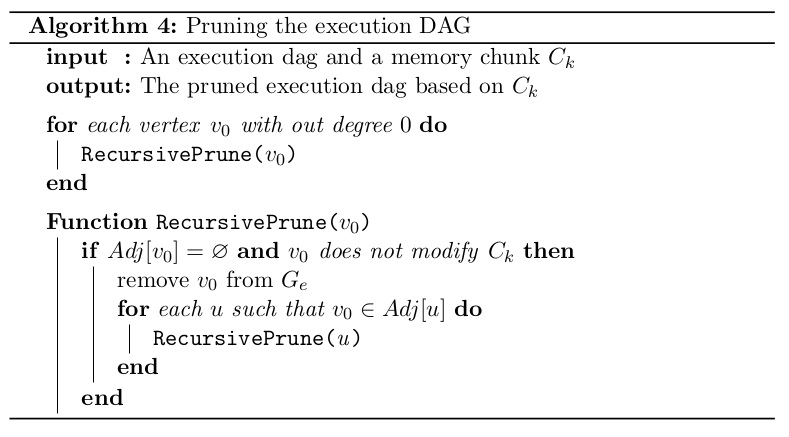
\includegraphics[width=17cm]{../img/Alg4s.png}
    \begin{algorithm}
        \DontPrintSemicolon
        \SetKwData{V}{$v_0$}\SetKwData{Graph}{$G_e$}\SetKwData{Chunk}{$C_k$}\SetKwData{Txns}{$T$}
        \SetKwFunction{RPrune}{RecursivePrune}
        \SetKwProg{Fn}{Function}{}{}
        \SetKwInOut{Input}{input}\SetKwInOut{Output}{output}
        \Input{An execution dag and a memory chunk \Chunk}
        \Output{The pruned execution dag based on \Chunk}
        \BlankLine
        \For{each vertex \V with out degree $0$}
        {
            \RPrune{\V}\;
        }
        \BlankLine
        \Fn{\RPrune{\V}}
        {
            \If{$Adj[\V] = \varnothing$ {\bf and} \V does not modify \Chunk}
            {
                remove \V from \Graph\;
                \For{each $u$ such that $\V \in Adj[u]$}
                {
                    \RPrune{u}\;
                }
            }
        }
        \caption{Pruning the execution DAG}\label{alg:prune_dag}
    \end{algorithm}

    If we choose chunks in a way that most transactions only modify memory locations of one chunk,
    likely the transactions of a block are divided between voting committees and are validated in parallel.

    Because the voting committees are selected by random sampling, by choosing large enough samples we can make sure
    that having multiple voting committees will not change the security properties of the Argennon agreement protocol.

    \section{Consensus}\label{sec:consensus}

    The consensus protocol of Argennon is similar to Algorand with a few minor improvements.

    \subsection{Estimating A User's Stake}\label{subsec:estimating-a-user's-stake}

    In a proof of stake system the influence of a user in the consensus protocol should be proportional to the amount
    of stake the user has in the system. Conventionally in these systems, for estimating a user's stake, we use the
    amount of native system tokens the user is holding. Unfortunately, one problem with this approach is that a
    strong attacker may be able to obtain a considerable amount of system tokens, for example by borrowing from a
    DEFI application, and use this stake to attack the system.

    To mitigate this problem, for calculating a user's stake at the time step \(t\), instead of using the raw ARG
    balance, we use the minimum of a \emph{trust value} the system has calculated for the user and the user's
    ARG balance:
    \[
        S_{u,t} = \min (B_{u,t}, Trust_{u,t})
    \]
    Where:
    \begin{itemize}
        \item \(S_{u,t}\) is the stake of the user \(u\) at the time step \(t\).
        \item \(B_{u,t}\) is the ARG balance of the user \(u\) at the time step \(t\).
        \item \(Trust_{u,t}\) is an estimated trust value for the user \(u\) at the time step \(t\).
    \end{itemize}

    The agreement protocol, at the time step \(t\), will use \(\sum_{u}S_{u,t}\) to determine the required
    number of votes for the confirmation of a block, and we let \(Trust_{u,t} = M_{u,t}\), where \(M_{u,t}\) is the
    exponential moving average of the ARG balance of the user \(u\) at the time step \(t\).

    In our system a user who held ARGs and participated in the consensus for a long time is more trusted
    than a user with a higher balance whose balance has increased recently. An attacker who has obtained a large
    amount of ARGs, also needs to hold them for a long period of time before being able to attack the system.

    For calculating the exponential moving average of a user's balance at the time step \(t\), we can use the following
    recursive formula:
    \[
        M_{u,t} = (1 - \alpha) M_{u,t-1} + \alpha B_{u,t} = M_{u,t-1} + \alpha (B_{u,t} - M_{u,t-1})
    \]
    Where the coefficient \(\alpha\) is a constant smoothing factor between \(0\) and \(1\) which represents the
    degree of weighting decrease, A higher \(\alpha\) discounts older observations faster.

    Usually an account balance will not change in every time step, and we can use older values of EMA for calculating
    \(M_{u,t}\): (In the following equations the \(u\) subscript is dropped for simplicity)
    \[
        M_{t} = (1 - \alpha)^{t-k}M_{k} + [1 - (1 - \alpha)^{t - k}]B
    \]
    Where:
    \[
        B = B_{k+1} = B_{k+2} = \dots = B_{t}
    \]
    We know that when \(|nx| \ll 1\) we can use the binomial approximation \({(1 + x)^n \approx 1 + nx}\). So, we can
    further simplify this formula:
    \[
        M_{t} = M_{k} + (t - k) \alpha (B - M_{k})
    \]

    For choosing the value of \(\alpha\) we can consider the number of time steps that the trust value of a user needs
    for reaching a specified fraction of his account balance. We know that for large \(n\) and \(|x| < 1\) we have
    \((1 + x)^n \approx e^{nx}\), so by letting \(M_{u,k} = 0\) and \(n = t - k\) we can write:
    \[
        \alpha =- \frac{\ln\left(1 - \frac{M_{n+k}}{B}\right)}{n}
    \]
    The value of \(\alpha\) for a desired configuration can be calculated by this equation. For instance, we could
    calculate the \(\alpha\) for a relatively good configuration in which \(M_{n+k} = 0.8B\) and \(n\) equals to the
    number of time steps of 10 years.

    In our system a newly created account will not have voting power for some time, no matter how high its
    balance is. While this is a desirable property, in case a large proportion of total system tokens are
    transferred to newly created accounts, it can result in too much voting power for older accounts. This may decrease
    the degree of decentralization in our system.

    However, this situation is easily detectable by comparing the total stake of the system with the total balance of
    users. If after confirming a block the total stake of the system goes too low and we have:
    \[
        \sum_{u}S_{u,t} < \gamma \sum_{u}B_{u,t}
    \]
    The protocol will perform a \emph{time shift} in the system: the time step of the system
    will be incremented for \(m\) steps while no blocks will be confirmed. This will increase the value of \(M_{u,t}\)
    for new accounts with a non-zero balance, giving them more influence in the agreement protocol.

    For calculating the value of \(m\) which determines the amount of time shift in the system, we should note that when
    \(B_{u,t} = B_{u, t-1} = B_u\), we can derive a simple recursive rule for the stake of a user:
    \[
        S_{u,t} = (1 - \alpha) S_{u,t-1} + \alpha B_u
    \]
    Therefore, we have:
    \[
        \sum_{u}S_{u,t} = (1 - \alpha) \sum_{u}S_{u,t - 1} + \alpha \sum_{u}B_u
    \]
    This equation shows that when the balance of users is not changing over time the total stake of the system is the
    exponential average of the total ARGs of the system. Consequently, when we shift the time for \(m\) steps, we can
    calculate the new total stake of the system from the following equation:

    \[
        \sum_{u}S_{u,t+m} = (1 - \alpha)^{m}\sum_{u}S_{u,t} + [1 - (1 - \alpha)^{m}]\sum_{u}B_u
    \]
    Hence, if we want to increase the total stake of the system from \(\gamma \sum_{u}B_u\) to \(\lambda \sum_{u}B_u\),
    we can obtain \(m\) from the following formula, assuming \(\alpha\) is small enough:
    \[
        m = \frac{1}{\alpha} \ln \left(\frac{1 - \gamma}{1 - \lambda}\right)
    \]


    \section{Smart Contract Oracle}\label{sec:smart-contract-oracle}

    A smart contract oracle is a full AVM emulator that keeps a full local copy of AVM memory and can emulate AVM
    execution without accessing a ZK-EDB. Smart contract oracles can be used for reporting useful information about
    \texttt{avmCall} transactions such as accessed AVM heap or code area locations, exact amount of execution cost,
    and so on.

\end{document}





    \chapter{The Argon Language}\label{ch:argon-lang}
    %! Author = aybehrouz

\lstset{
    language=Java,
    morekeywords={main, initialize, constructor, external, virtual, Map, Account, signature, overrides, is, string},
    basicstyle=\small\sffamily,
    columns=fullflexible,
%   keywordstyle=\bfseries,
    breaklines=true,
    showstringspaces=false,
    mathescape
}

\section{Introduction}\label{sec:introduction2}

The Argon programming language is a class-based, object-oriented language designed for writing Argennon smart
contracts. The Argon programming language is inspired by Solidity and is similar to Java, with a number of aspects
of them omitted and a few ideas from other languages included. Argon is designed to be fully compatible with
the Argennon Virtual Machine and be able to use all advanced features of the Argennon blockchain.

Argon applications (i.e.\ smart contracts) are organized as sets of packages. Each package has its own set of names
for types, which helps to prevent name conflicts. Every package can contain an arbitrary number of classes.
Every Argon application is required
to have exactly one \texttt{main} method and one \texttt{initialize} method. The \texttt{main} method is the
only method of an Argon application which would be called by other smart contracts.

The \texttt{main} method is required to have a single parameter named \texttt{request}. The type of this parameter
should be \texttt{RestRequest} or \texttt{HttpRequest}. The return value of the \texttt{main} function needs to be a
\texttt{RestResponse} or \texttt{HttpResponse}.


\section{Features Overview}\label{sec:features-overview}

\subsection{Access Level Modifiers}\label{subsec:access-level-modifiers}

Access level modifiers determine whether other classes can use a particular field or invoke a particular method.

\begin{center}
    \begin{tabular}{lllll}
        \hline
        & Class & Package & Subclass & Program \\
        \hline
        private   & yes   & no      & no       & no  \\
        protected & yes   & no      & yes      & no  \\
        package   & yes   & yes     & yes      & no  \\
        public    & yes   & yes     & yes      & yes \\
        \hline
    \end{tabular}\label{tab:table}
\end{center}


\begin{lstlisting}[frame=TB, float, title=A simple Argon application,label={lst:code1}]
public class MirrorToken {
    private static SimpleToken token;
    private static SimpleToken reflection;

    // `initialize` is a special static method that is called by the AVM after the code of a contract
    // is stored in the AVM code area.
    public static void initialize(double supply1, double supply2) {
        // `new` does not create a new smart contract. It just makes an ordinary object.
        token = new SimpleToken(supply1);
        reflection = new SimpleToken(supply2);
    }
    // `main` is the only method of the application (i.e. smart contract) that can be called
    // by other applications. Every application should have exactly one main method defined
    // in some class. Alternatively, the keyword `dispatcher` could be used instead of `main`.
    public static RestResponse main(RestRequest request) {
        RestResponse response = new RestResponse();
        if (request.pathMatches("/balances/{user}")) {
            Account sender = request.getParameter<Account>("user");
            if (request.operationIsPUT()) {
                sender.authorize(request.toMessage(), request.getParameter<byte[]>("sig"));
                Account recipient = request.getParameter<Account>("to");
                double amount = request.getParameter<double>("amount");
                token.transfer(sender, recipient, amount);
                reflection.transfer(recipient, sender, Math.sqrt(amount));
                return response.setStatus(Http.Status.OK);
            } else if (request.operationIsGET()) {
                response.append<double>("balance", token.balanceOf(sender));
                response.append<double>("reflection", reflection.balanceOf(user));
                return response.setStatus(Http.Status.OK);
            } else {
                return response.setStatus(Http.Status.MethodNotAllowed);
            }
        }
    }
}

package class SimpleToken {
    private Map(Account -> double) balances;

    // The visibility of a member without an access modifier will be the package level.
    constructor(double initialSupply) {
        // initializes the object
    }

    void transfer(Account sender, Account recipient, double amount) {
        if (balances[sender] < amount) throw("Not enough balance.");
        // implements the required logic...
    }
    // implements other methods...
}
\end{lstlisting}

\subsection{Shadowing}\label{subsec:shadowing}

If a declaration of a type (such as a member variable or a parameter name) in a particular scope (such as an
inner block or a method definition) has the same name as another declaration in the enclosing scope, it will
result in a compiler error. In other words, the Argon programming language does not allow shadowing.




    \chapter{Persistence Layer}\label{ch:persistance}
    %! Author = aybehrouz


The Argennon Virtual Machine has two persistent memory areas: \emph{method area}, and \emph{heap}. Method area stores
method byte codes\footnote{also it stores constant area blocks.}, and heap stores memory chunks. Both of these
data elements, methods and chunks, can be considered as continuous pieces of byte addressable memory
which we shall call \emph{objects} throughout this chapter.

In the AVM persistence layer, similar objects are clustered together and constitute a bigger data element which we call a
\emph{page}.\footnote{we avoided calling them a cluster, because usually a cluster refers to a \emph{set}. AVM object
clusters are not sets. They are ordered lists, like a page containing an ordered list of words or sentences.}
A page is an ordered list of an arbitrary number of objects, which their order reflects the order they were added to
the page:
\[
    P = (O_1,O_2,\dots,O_n),\quad i < j \; \Leftrightarrow \; \textrm{$O_i$ was added before $O_j$}
\]

A page of the AVM storage should contain objects that have very similar access pattern. We expect that when a page
is needed for validating a block, almost all of its objects are needed. We also prefer that the objects of the page
are needed for the same access type. In other words, the objects of a page are chosen in a way that
for validating a block, we usually need to either read all of them or modify\footnote{and probably read.} all of them.

Pages of the AVM storage space are persisted using updatable zero-knowledge elementary databases (ZK-EDB). Argennon
has three zero-knowledge databases. \emph{Staking} database which stores all the data that is associated with
the Argennon agreement protocol. \emph{Method} database which stores the AVM method area, and \emph{Heap} database which
stores the AVM heap. The commitment of these three ZK-EDBs are included in every block of the Argennon blockchain.

We consider the following properties for a ZK-EDB:
\begin{itemize}
    \item The ZK-EDB contains a mapping from a set of keys to a set of values.
    \item Every state of the database has a commitment \(C\).
    \item The ZK-EDB has a method \((D, \pi) = get(x)\), where \(x\) is a key and \(D\) is the associated data
    with \(x\), and \(\pi\) is a proof.
    \item A user can use \(C\) and \(\pi\) to verify that \(D\) is really associated with \(x\), and \(D\) is not
    altered. Consequently, a user who can obtain \(C\) from a trusted source does not need to trust the ZK-EDB\@.
    \item Having \(\pi\) and \(C\) a user can compute the commitment \(C'\) for the database in which \(D'\) is
    associated with \(x\) instead of \(D\).
\end{itemize}

Every page of the AVM storage is stored with an index as its key: \texttt{pageIndex}. The \texttt{pageIndex} is
required to be smaller than a certain value determined by the
protocol.\footnote{this facilitates the usage of ZK-EDBs that use vector commitments.}
Therefore, the AVM clustering algorithm tries to reuse indices and keep the number of used indices as low as
possible.

In Argennon \emph{light} nodes do not keep a full copy of the AVM storage and for emulating the Argennon Virtual Machine
( i.e.~validating transactions) they need to connect to a ZK-EDB and retrieve the required pages.
Because light node need to be able to validate block certificates, they usually cache a large part of the staking
database, and keep their cache updated to make sure they can keep themselves in sync with the blockchain.

The commitments of the AVM databases are dependant to the clustering of data objects. So, the clustering algorithm of
the AVM storage has to be a part of the Argennon agreement protocol. Clustering of objects is one of the
tasks that a block proposer performs in Argennon.

Every block of the Argennon blockchain contains a set of \emph{clustering directives}. These directives
can only modify pages that were used for validating the block, and can
include directives for moving an object from one page to another or directives specifying which pages will contain
the newly created objects. These directives will always be run by nodes at the end of block validation.

A block proposer usually obtains clustering directives from a third party source who enjoys a considerable amount of
computational power. This federated approach does not affect Argennon security, because the integrity of a
database can not be altered by clustering directives. Those
directives can only affect the performance of the argennon blockchain, and directives of a single block can
not change the performance much.



    \chapter{Networking Layer}\label{ch:networking}
    \section{Normal Mode}\label{sec:normal-mode}
    Unlike conventional blockchains, Argennon does not use a P2P network architecture. Instead, it uses a
    client-server topology, based on a permission-less list of ZK-EDB servers. ZK-EDB servers are a
    crucial part of the Argennon ecosystem, and they form the backbone of the Argennon networking layer.
    \note{not yet written...}


    \section{Censorship Resilient Mode}\label{sec:cens-res-mode}
    \note{not yet written...}


    \chapter{The Argennon Blockchain}\label{ch:argennon-blockchain}
    %! Author = aybehrouz

\section{Applications}\label{sec:applications}

An Argennon application or a smart contract is a collection of method bytecodes and heap chunks that are stored in
the AVM storage, identified by a unique application identifier. An application identifier, \texttt{applicationID}, is
a unique prefix code generated by the \emph{applications} prefix tree. (See Section~\ref{sec:identifiers}.)

An application identifier can
be considered as the address of an application and has the following standard symbolic representation:
\begin{verbatim}
<application-id> ::= <decimal-prefix-code>
<decimal-prefix-code> ::= <dec-num>"."<decimal-prefix-code> | <dec-num>
\end{verbatim}
where \texttt{<dec-num>} is a normal decimal number between $0$ and $255$.

For example \texttt{21.255.37}, \texttt{0} and \texttt{1.0.0.0.0}, are valid application addresses.

Argennon has two special smart contracts: the \emph{root smart contract}, also called the \emph{root application}, and
the \emph{ARG smart contract}, which is also called the Argennon smart contract or the \emph{ARG application}.

\subsection{The Root Application}\label{subsec:the-root-app}

The root application or the root smart contract, with \texttt{applicationID = 0}, is a privileged smart contract
responsible for installation/uninstallation of other smart contracts. The Argennon root smart contract
performs three main operations:

\begin{itemize}
    \item Installation of AVM smart contracts and determining the update policy of a smart
    contract: if the contract is updatable or not, which accounts can update or uninstall the contract, and so
    on.
    \item Removing AVM smart contracts.
    \item Updating an AVM smart contract (if allowed).
\end{itemize}

The root smart contract is a mutable smart contract and can be updated by the Argennon governance system.
(See Section~\ref{sec:adags})

\subsection{The ARG Application}\label{subsec:the-arg-app}

The ARG application or the ARG smart contract,
with \texttt{applicationID = 1}, controls the ARG token, the main
currency of the Argennon blockchain. This smart contract also manages a database of public keys and
handles signature verification.

The ARG smart contract is a mutable smart contract and can be updated by the Argennon governance system.


\section{Accounts}\label{sec:accounts}

Argennon accounts are entities defined inside the ARG smart contract.
Every Argennon account is uniquely identified by a prefix code generated using \emph{accounts} prefix
tree. (See Section~\ref{sec:identifiers}) An account
identifier can be considered as the address of an account and has the following standard symbolic representation:
\begin{verbatim}
<account-id> ::= <hex-prefix-code>
<hex-prefix-code> ::= "0x"<hex-num>"."<hex-prefix-code> | "0x"<hex-num>
\end{verbatim}
where \texttt{<hex-num>} is a hexadecimal number between $0$ and $255$, using lower case
letters \texttt{[a-f]} for showing digits greater than $9$.

For example \texttt{0x24.0xff.0xda}, \texttt{0x0} and \texttt{0x3.0xa0.0x0.0x0}, are valid standard symbolic
representations of account addresses.

A new account can be created by invoking \texttt{createAccount} method from the Argennon smart contract. For creating
a new account two public keys need to be provided by the caller and registered in the Argennon smart contract.
One public key will be used for issuing digital signatures, and the other one will be used for voting. The
provided public keys need to meet certain cryptographic requirements,\footnote{Argennon uses Prove
Knowledge of the Secret Key (KOSK) scheme.} and can not be already registered in the system.

If the owner of the new account is an application, the \texttt{applicationID} of the owner will be registered in the
ARG smart contract and no public keys are needed. An application can own an arbitrary number of accounts.

\note{Explicit key registration enables Argennon to decouple cryptography from the blockchain design. In this way,
    if the cryptographic algorithms used become insecure for some reason, for example because
    of the introduction of quantum computers, they could be easily upgraded.}


\section{Transactions}\label{sec:transactions}

Every Argennon transaction consists of two \texttt{i\_invoke\_dispatcher} instructions, the first instruction always
transfers the proposed fee of the transaction in ARGs from a sender account to the fee sink accounts, and
the second performs the requested operation. If the first instruction fails, the transaction will not be added to
the Argennon blockchain.

Users interact with AVM smart contracts using
the second \texttt{i\_invoke\_dispatcher} instruction of a transaction.
Transferring all assets, including ARG, is done by that instruction.

The \texttt{i\_invoke\_dispatcher} instruction invokes the \texttt{dispatcher} method of a smart contract. Every AVM
smart contract has a \texttt{dispatcher} method, and the Argennon protocol requires
the \texttt{dispatcher} method to accept an HTTP request as its argument and
return an HTTP response.

As a result, every Argennon transaction contains two HTTP requests. In addition to these HTTP requests, the
transaction is required to contain a resource declaration object, specifying the maximum amount of resources
it needs for execution.

\note{Argennon smart contracts use HTTP as the application protocol and they are advised to have a RESTful API design.}

\subsection{Resource Declaration}\label{subsec:resource-declaration}

Every Argennon transaction is required to specify a cap for all the resources it needs. This
includes memory, network and processor related resources. When a transaction reaches one of its
pre-declared resource caps, executing any AVM instruction which uses that resource, will result in an AVM exception.

As we know, every Argennon transaction consists of two \texttt{i\_invoke\_dipatcher} instructions. The first
instruction is always considered as a \emph{free} instruction and resources spent during its execution
session will not be counted. As a result, only the second instruction could fail due to exceeding resource limits.

The Argennon protocol defines an execution cost for
every AVM instruction, reflecting the amount of resources its emulation needs. Every
transaction is required to specify two maximum execution costs: \texttt{maxInternalCost}
and \texttt{maxExternalCost}. The \emph{external} execution cost of a transaction is the \textbf{overall} cost of its
\texttt{invoke\_dispatcher} and \texttt{invoke\_later} instructions,\footnote{By overall cost, we mean the execution
cost needed for reaching the next instruction.} and the remaining execution cost will be considered as
the \emph{internal} cost. If a transaction reaches one of its maximum costs, executing any instruction which has
that type of cost, will throw an AVM exception.

\note{When a transaction reaches its \texttt{maxExternalCost}, it can still keep executing
its own code, while it can not call other smart contracts.
This way the execution cost of a smart contract is completely decoupled from the
smart contract it calls, and a malicious contract can not make its invoker fail unconditionally
by using infinite loops.}

Also, Argennon transactions are required to specify what heap or code area addresses they will access. This will
enable validators to parallelize transaction validation as we will see in Section~\ref{sec:concurrency}. A transaction
that tries to access a memory location that is not in its access list, will be rejected.
Users could use off-chain \emph{smart contract oracles} to predict the list of memory locations their transactions need.

A smart contract oracle is a full AVM emulator that keeps a full local copy of the AVM storage and can emulate AVM
execution without accessing a ZK-EDB server. Smart contract oracles can be used for reporting useful information about
Argennon transactions such as accessed AVM heap or code area locations, exact amount of execution cost,
and so on.

Every Argennon transaction is required to provide the following information as an upper bound for the
resources it needs:

\begin{itemize}
    \item Maximum internal execution cost
    \item Maximum external execution cost
    \item A list of heap/code-area locations for reading
    \item A list of heap locations for writing
    \item A list of heap chunks it will deallocate (if any)
    \item A list of methods it will delete (if any)
    \item Number and size of heap chunks it will allocate (if any)
    \item Number and size of method bytecodes it will allocate (if any)
\end{itemize}

If a transaction tries to violate any of these predefined limitations, it will be considered failed, and the network
can receive the proposed fee of that transaction.

\subsection{Authorization}\label{subsec:txn-auth}

Argennon transactions do not have a sender. The authorization of the requested operation is always done by checking the
digital signatures that are provided as a part of the HTTP request to the \texttt{dispatcher} method.

While every block of the Argennon blockchain stores the commitment of the transaction list, Argennon does not enforce
storage of the transaction history. To be able to detect replay attacks, we require
every signature that a user creates to have a nonce. This nonce consists of the issuance round of the signature
and a sequence number: \texttt{(issuance,\ sequence)}. When a user creates more than one signature in a round, he
must sequence his signatures starting from 0 (i.e.~the sequence number restarts from 0 in every round). We define
a maximum lifetime for signatures, so a signature is invalid if \texttt{currentRound - issuance > maxLifeTime} or
if a signature of the same user with a bigger or equal nonce is already used
(i.e.~is recorded in the blockchain). A nonce is bigger than another nonce if it has an older issuance. If two
nonces have an equal issuance, the nonce with the bigger sequence number will be considered bigger.

To be able to detect invalid signatures, we keep the maximum nonce of used digital signatures per user. This information
is stored in the ARG smart contract and when the difference between \texttt{issuance} component of the nonce and
the current round becomes bigger than the maximum allowed lifetime of a signature, it can be safely
deleted.\footnote{in some conventional
blockchains, the nonce data can never be deleted, even if the account has zero balance and is no longer used.}


\begin{lstlisting}[language=python, frame=TB, float, title=An Argennon transaction in YAML format,label={lst:txn-example}]
---
fee: |
    PUT /balances/0x73.0xa2?to=fee&amount=0.26&sig=5b73CbmwQNRC7fWUY15 HTTP/1.1
call: |
    POST httpb://bac.argennon.net/54.189.21/proposals HTTP/1.1
    Content-Type: application/json; charset=utf-8
    Content-Length: 69

    {
        "name": "Grant Proposal",
        "recipient": "0x24.0x8f.0x29.0xa1",
        "amount": 25000,
        "sig"= "2a36Gtrw249wQCD70nWY49d"
    }
caps:
    internal: 2500000 # maximum number of AVM execution clocks
    external: 1000000
    read: [(2654,3),(15642,0),(15642,1),(15642,3)]
    write: [(15642,0),(20154,0),(20154,1)]
\end{lstlisting}

\subsection{Transaction Fee}\label{subsec:fee}

Every Argennon transaction is required to pay two types of fees: execution fee, which is paid for executing the
transaction, and storage fee, which is paid for the amount of storage the transaction allocates.

A transaction pays
its fees by providing digital signatures of one or more accounts, authorizing the transfer of the amount of fee in
ARG from one or more accounts to the fee sink accounts, and the fee is transferred by the first
\texttt{i\_invoke\_dispatcher} instruction of the transaction.

\note{An Argennon transaction always pays all of its proposed fee, no matter how much of its predefined resources
were not used in the final emulation. This will incentivize users to report the resource usage of their
transactions more accurately.}




    \section{Blocks}\label{sec:blocks}
    %! Author = aybehrouz

The Argennon blockchain is a sequence of blocks. Every block represents an ordered list of transactions, intended to be
executed by the Argennon Virtual Machine. The first block of the blockchain, the \emph{genesis} block, is a spacial
block that fully describes the initial state of the AVM. Every block of the Argennon blockchain thus corresponds to a
unique AVM state which can be calculated deterministically from the genesis block.

A block of the Argennon blockchain contains the following information:

\begin{center}
    \begin{tabular}{||c||}
        \hline
        \textbf{Block} \\ [0.5ex]
        \hline\hline
        commitment to the staking database            \\ [1.2ex]
        commitment to the method database             \\ [1.2ex]
        commitment to the heap database               \\ [1.2ex]
        commitment to the set of transactions         \\ [1.2ex]
        a consecutive list of block certificates issued     \\
        by validators' committee (if any)           \\ [1.2ex]
        clustering directives                         \\ [1.2ex]
        random seed                                   \\ [1.2ex]
        previous block hash                           \\ [1.2ex]
        \hline
    \end{tabular}
\end{center}

\subsection{Block Validation}\label{subsec:block-validation}

Having the previous AVM state, the transaction list and the clustering directives of a block, a node can calculate
commitments to the staking, method and heap databases of the current block by emulating the AVM execution. If the
node can obtain the previous block information from a trusted source, it does not need to have a trusted local
copy of the AVM state,
and it can reliably retrieve the required storage pages from a ZK-EDB server. We call this type of block verification
\emph{conditional} block validation. This validation is conditional because the validity of the current block is
conditioned on the validity of the previous block.

Interestingly, conditional block validation of multiple blocks can be done in parallel. If a node has enough bandwidth
and computational resources, it can conditionally verify any number of blocks from a previously created blockchain
simultaneously and in parallel. As we will see in Section~\ref{subsec:validators-committee}, this property plays an
important role in the Argennon consensus protocol.

To some extent, conditional validation of a single block could be parallelized as well. Many transactions
in a block are actually independent and the order of their execution does not
matter. These transactions can be safely validated in parallel. Section~\ref{sec:concurrency} further
develops this concept.


\subsection{Block Certificate}\label{subsec:block-certificate}

An Argennon block certificate is an aggregate signature of some predefined subset of accounts. This predefined subset
is called the certificate committee and their signature ensures that the certified block is conditionally
valid given the validity of some previous block.

Argennon uses BLS aggregate signatures to represent block certificates. To better understand block certificates and
the Argennon consensus protocol, we need to briefly review the BLS signature scheme and its aggregation mechanism.

The BLS signature scheme operates in a prime order group and supports simple threshold signature generation,
threshold key generation, and signature aggregation. To review, the scheme uses the following ingredients:

\newcommand{\G}{\mathbb{G}}
\newcommand{\Z}{\mathbb{Z}}
\newcommand{\adv}{{\cal A}}
\newcommand{\bdv}{{\cal B}}
\newcommand{\deq}{\mathrel{\mathop:}=}
\newcommand{\SK}{\mathit{sk}}
\newcommand{\PK}{\mathit{pk}}
\newcommand{\C}{\mathit{cert}}
\newcommand{\APK}{\mathit{apk}}
\newcommand{\DPK}{\mathit{\Delta pk}}
\newcommand{\MM}{\mathcal{M}}
\newcommand{\xwedge}{\, \operatorname{\text{$\wedge$}}\, }
\newcommand{\abs}[1]{\lvert #1 \rvert}
\newcommand{\Hm}{H_0}
\newcommand{\Hpk}{H_1}
\newcommand{\qHpk}{Q_{\Hpk}}
\newcommand{\qHm}{Q_{\Hm}}
\newcommand{\qsig}{Q_{\text{sig}}}

\begin{itemize}
    \item An efficiently computable \emph{non-degenerate} pairing $e:\G_0 \times \G_1 \to \G_T$
    in groups $\G_0$, $\G_1$ and $\G_T$ of prime order $q$. We let $g_0$ and $g_1$ be generators
    of $\G_0$ and $\G_1$ respectively.
    \item A hash function $H_0: \mathcal{M} \rightarrow \mathbb{G}_0$, where $\mathcal{M}$ is the message space.
    The hash function will be treated as a random oracle.
\end{itemize}

The BLS signature scheme is defined as follows:

\begin{itemize}
    \item $\textbf{KeyGen}()$: choose a random $\alpha$ from $\Z_q$ and set $h \gets g_1^\alpha \in \G_1$.
    output $\PK \deq (h)$ and $\SK \deq (\alpha)$.
    \item $\textbf{Sign}(\SK, m)$: output $\sigma \gets \Hm(m)^\alpha \in \G_0$.
    The signature $\sigma$ is a \emph{single} group element.
    \item $\textbf{Verify}(\PK,m,\sigma)$: if $e(g_1, \sigma) = e\big(\PK,\ \Hm(m)\big)$  then output "accept",
    otherwise output "reject".
\end{itemize}

Given triples $(\PK_i,\ m_i,\ \sigma_i)$ for $i=1,\ldots,n$,
anyone can aggregate the signatures $\sigma_1,\ldots,\sigma_n \in \G_0$
into a short convincing aggregate signature $\sigma$ by computing
\begin{equation}
    \label{eq:agg}
    \sigma \gets \sigma_1 \cdots \sigma_n \in \G_0\ .
\end{equation}
Verifying an aggregate signature $\sigma \in \G_0$ is done by checking that
\begin{equation}
    \label{eq:aggdiff}
    e(g_1, \sigma) = e\big(\PK_1,\ \Hm(m_1)\big) \cdots e\big(\PK_n,\ \Hm(m_n)\big)\ .
\end{equation}
When all the messages are the same ($m = m_1 = \ldots = m_n$), the verification relation~\eqref{eq:aggdiff} reduces to
a simpler test that requires only two pairings:
\begin{equation}
    \label{eq:aggsame}
    e(g_1, \sigma) = e\Big(\PK_1 \cdots \PK_n,\ \Hm(m)\Big)\ .
\end{equation}
We call $\APK=\PK_1 \cdots \PK_n$ the aggregate public key.

To defend against \emph{rogue public key} attacks, Argennon uses Prove Knowledge of the Secret Key (KOSK) scheme. As we
explained in Section~\ref{sec:accounts}, when an account is created its public keys need to be registered in
the ARG smart contract. Therefore, the KOSK scheme can be easily implemented in Argennon.

Because it is not usually possible to collect the signatures of all members of a certificate committee, an Argennon
block certificate essentially is an Accountable-Subgroup Multi-signature (ASM). Argennon uses a simple ASM scheme
based on BLS aggregate signatures.

Argennon block certificates constitute an ordered sequence based on the order of blocks they certify. If we show
the certificate of committee $C$ for the $i$-th block\footnote{note that the $i$-th block certificate is not
necessarily the certificate of the $i$-th block.} with $\C_i$, and the set of signers
with $S_i$, then the block certificate $\C_i$ can be considered as a tuple:
\begin{equation}
    \C_i=(\sigma_i,\ C-S_{i})\label{eq:cert}\ ,
\end{equation}
where $\sigma_i$ is the aggregate signature issued by $S_i$.

The aggregate public key of the certificate can
be calculated from:
\begin{equation}
    \APK_i=\APK_C\APK_{C-S_i}^{-1}\label{eq:aggCertPK}\ ,
\end{equation}
where $\APK_{A}$ shows the aggregate public key of all accounts in $A$.

Alternately we can use $\APK_{i-1}$ to calculate the aggregate public key:
\begin{equation}
    \APK_i=\APK_{i-1}\APK_{S_i-S_{i-1}}\APK_{S_{i-1}-S_i}^{-1}\ .\label{eq:aggPK-2}
\end{equation}

When an Argennon account is created, both its $\PK$ and $\PK^{-1}$ is registered in the ARG smart contract, so the
inverse of any aggregate public key can be easily computed.\footnote{since the group operator of a cyclic
group is commutative, we have $(ab)^{-1}=a^{-1}b^{-1}$.}




    \section{Consensus}\label{sec:consensus}
    %! Author = aybehrouz

The credibility of a block of the Argennon blockchain is determined by the certificates it has received
from different sets of users, knows as committees. There are two primary type of certificate committees in
Argennon: the committee of \emph{delegates} and the committee
of \emph{validators}. Argennon has \emph{one} committee of delegates and $m$ committees of validators.

The committee of delegates issues a certificate for every block of the Argennon blockchain, and each
committee of validators issues a certificate every $m$ blocks. A validators' committee will
certify a block only if it has already been certified by the committee of delegates. Every committee of validators has
an index between $0$ and $m - 1$, and it issues a certificate for block number $n$, if $n$ modulo $m$ equals
the committee index.

Every block of the Argennon blockchain needs a certificate from both the committee of delegates and
the committee of validators. A block is considered final after its \textbf{next} block receives \textbf{both} of
its certificates. In Argennon as long as more than half of the total stake of validators is controlled by honest users,
the probability of discarding a final block is near zero even if all the delegates are malicious.

In addition to primary committees, Argennon has several community driven committees. Certificates of these
committees are not required for block finality, but they could be used by members of the
validators' committee to better decide about the validity of a block.

When an anomaly is detected in the consensus mechanism, the \emph{recovery} protocol is initiated by validators. The
recovery protocol is designed to be resilient to many types of attacks in order to be able to restore the normal
functionality of the system.

\subsection{The Committee of Delegates}\label{subsec:the-committee-of-delegates}

The committee of delegates is a small committee of trusted delegates, elected by Argennon users through the
Argennon Decentralized Autonomous Governance system (ADAGs\footnote{pronounced \textipa{/eI-dagz/}.}).
At the start of the Argennon mainnet, this committee will have
five members, and later its size could be changed by the ADAGs in a procedure described
in Section~\ref{sec:adags}.

The committee of delegates is responsible for creating new blocks of the Argennon blockchain, and it issues a
certificate for every block of the Argennon blockchain. A certificate needs to be signed
by \textbf{all} of the committee members in order to be considered valid.

Besides the main delegates' committee, a reserve committee of delegates consists of three members is elected by users
either through the ADAGs or by \emph{emergency agreement} during the recovery protocol. In case the main committee
fails to generate new blocks or behaves maliciously, the task of
block generation will be assigned to the reserve committee until a new main delegates' committee is elected
through the ADAGs.

Usually, the delegates are large organizations, and they have enough computational resources to generate blocks
very fast. However, a block is not completely final if it does not have the certificate of its validators.
A certified block by the delegates will not be accepted by the network, if the last block certified by
the validators is behind it more than a certain number of blocks.

The committee of delegates may use any type of agreement protocol to reach consensus on the
next block. Usually a very simple and fast protocol can do the job: one of the members
is randomly chosen as the proposer, and other members vote "yes" or "no" on the proposed block.

If one of the delegates lose its network connectivity, no new blocks can be generated. For this reason,
the delegates should invest on different types of communication infrastructure, to make sure they never lose
connectivity to each other and to the Argennon network.

\subsection{Validators}\label{subsec:validators-committee}

The Argennon protocol calculates a stake value for every account, which is an estimate of a user's stake in the
system, and is measured in ARGs. Any account whose stake value is higher than
\texttt{minValidatorsStake} threshold is considered a \emph{validator}.
The \texttt{minValidatorsStake}
threshold is determined by the ADAGs, but it can never be higher than $500$ ARGs.

Every \texttt{committeeLifeTime} number of blocks, randomly $m$ committees are selected from
validators, in a way that the total stakes of committees are almost equal, and every
account is a member of \textbf{at least} one committee.

Every validator has a status which can be either \texttt{online} or \texttt{offline}.
This status is stored in the ARG smart contract and is a part of the staking database. A validator can change
his status through a method invocation
from the ARG smart contract. When an account sets its status to \texttt{offline}, it receives a small reward, and
it can not change it back to \texttt{online} for \texttt{statusCoolDown} number of blocks.

\note{When a validator changes his status, the change has no effect until the block containing the status
change transaction gets certified by his committee.}

A block certificate issued by some members of a validators' committee is considered valid, if according to
the staking database of the previous block \textbf{certified by the same committee}, we have:\footnote{If we calculate
the stake values based on the previous block a malicious committee can select the validators of the next block.}
\begin{itemize}
    \item The total stake of \texttt{online} members of the committee is higher than \texttt{minOnlineStake} fraction
    of the total stake of the committee. This threshold can be changed by the ADAGs, but it can never be lower
    than $2/3$.
    \item All signers of the certificate have \texttt{online} status.
    \item The sum of stake values of the certificate signers is higher than $3/4$ of the total stake
    of the committee members that have \texttt{online} status.
\end{itemize}

The delegates can generate blocks very fast. Therefore, the Argennon blockchain always has an
unvalidated part, which contains blocks that have a certificate from the committee of delegates but have not
yet received a certificate from the validators.

As we mentioned before, the block with height $n$ needs a certificate from the committee of
validators with index $n$ modulo $m$. To decide about signing the certificate of a block which already has
a certificate from the delegates, a validator checks the conditional
validity\footnote{See Section~\ref{subsec:block-validation}} of the block, and
if the block is valid he issues
an "accept" signature. If the block is invalid, he initiates the recovery protocol. The validator will broadcast the
certificate \textbf{only after} he sees the certificate of the validators of the previous block.
Some validators may also require seeing a certificate from
some community driven committee. An honest validator never signs a certificate for two different blocks with the
same height.

So in Argennon, the block validation by committees is performed in parallel, and validators
do not wait for seeing the certificate of the previous block validators to start transaction validation. On the
other hand, the block certificates are published and broadcast sequentially. A validator does not publish its
certificate if the certificate of the previous block has not been published yet. This ensures that an invalid
fork made by malicious delegates will not receive any certificates from validators.

The value of $m$ is determined by the ADAGs. but it can never be higher than $25$. This way, it is guaranteed
that on average, any block of the Argennon blockchain is validated by at least $0.02$ of the total ARG supply.

block certificates issued by committees of validators are included in the blocks of the Argennon blockchain.
A block can contain multiple certificates, provided that
those certificates belong to consecutive blocks.

\subsection{Status Blocks}\label{subsec:status-blocks}

If according to the staking database of block $n$, the total online stake of the committee with index $n$ modulo $m$ is
lower than \texttt{minOnlineStake} threshold, the block $n + m$ can never be certified by validators.

To prevent blockchain from halting in such situations, the protocol performs a predefined partial
reshuffling of committee members.
In this reshuffling which is based on the block random seed, some online members from other committees will
be moved to the committee without enough online stake to make it active again.

If the reshuffling can not solve the problem due to low total online stake, the protocol requires the next block
of the blockchain to be a special \emph{status block}. A status block is a special block which can only contain
status change transactions. The status block need to be certified by the delegates and by 2/3 of the total stake of
validators. The \texttt{online}/\texttt{offline} status of validators will not be considered in the validity of
the status block certificate.\footnote{Theoretically at the status block, the total online stake of the system could
be very low. Therefore, the status block should not be certified only by online stake.} After applying
the transactions of the status block, the total online stake of all committees of validators
must go higher than \texttt{minOnlineStake} threshold.

\subsection{Signature Aggregation}\label{subsec:sig-agg}

In Argennon, signature aggregation is mostly performed by ZK-EDB servers. To distribute the aggregation workload
between different servers, Every committee of validators is divided into pre-determined groups, and each ZK-EDB
server is responsible for signature aggregation of one group. To make sure that there is enough redundancy, the
total number of groups should be less than the number of ZK-EDB servers and each group should be assigned to
multiple ZK-EDB servers.

Any member of a group knows all the servers that are responsible for signature aggregation of his group. When a member
signs a block certificate, he sends his signature to \textbf{all} the severs that aggregate the signatures of his group.
These servers aggregate the signatures they receive and then send the aggregated signature to the delegates.
Furthermore, the delegates aggregate these signatures to produce the final block certificate
and then include it in the next block.

The role of the delegates in the signature aggregation is limited. The important part of the work is done by ZK-EDB
servers. As long as there are enough honest ZK-EDB servers, the network will be able to perform signature aggregation
even if the delegates are malicious.

\subsection{The Recovery Protocol}\label{subsec:recovery}

The recovery protocol is a resilient protocol designed for recovering the Argennon blockchain from critical situations.
In the terminology of the CAP theorem, the recovery protocol is designed to choose consistency over availability,
and is not a protocol supposed to be executed occasionally. Ideally this protocol should never be used
during the lifetime of the Argennon blockchain.

The recovery protocol can recover the functionality
of the Argennon blockchain as long as more than 2/3 of the total stake of the system is controlled by honest users
and any network partition resolves after a finite amount of time. The recovery protocol uses two main emergency
procedures to recover the functionality of the Argennon blockchain: \emph{emergency forking} and \emph{emergency
agreement} protocol.

\subsubsection{Emergency Forking}

The reserve committee of delegates is able to fork the Argennon blockchain, if it receives a valid fork request
from the validators.
This fork needs to be confirmed by validators and can not discard any blocks that has been already certified
by validators.
A valid fork request is an unexpired request signed by more than half of the
total \texttt{online} stake of the validators.

For forking at block $b$, the reserve committee of delegates
makes a special \emph{fork block} which only contains a valid fork request, and its parent is the block $b$.
The height of the fork block is
$b + 1$ so it needs a valid certificate from the committee of validator with the index $b+1$ modulo $m$.

For signing a fork block, a validator ensures that the block is signed by the reserve committee and contains
a valid fork request. The parent of the fork block does not necessarily need a validators' certificate. If the
parent does not have a certificate, the validator checks the certificate of the block before the parent and
the conditional validity of the parent instead. This enables the reserve committee
to recover the liveliness of
the blockchain in a situation where a malicious committee has generated multiple blocks at the same height.

A validator always choose a valid fork block over a block of the main chain. However, as we mentioned before,
a validator never signs a certificate for two different blocks with the same height. Consequently, if a validator
has already signed the block $b$ of the main chain, he will not sign the fork block and vice versa.

When the fork block is broadcast, it is possible that the validators of the committee with index $b+1$ modulo $m$
get divided between the fork block and the block $b+1$ of the main chain, in a way that no block gets enough validators.
This will cause the blockchain to halt. To prevent this, the protocol allows the reserve delegates to revoke a
fork block. After a fork block
is revoked, the validators who voted for it are allowed to vote for another block with the same
height.

To revoke a fork block with height $b+1$, the delegates need to seal the fork by adding a special
\emph{seal block} after the fork block.\footnote{The parent of the seal block must be the fork block.} The seal block
has the height $b+2$ and needs to be certified by the validators' committee with the
index $b+2$ modulo $m$. The fork block is considered revoked only after the seal block is certified by the validators.

The seal block is not a normal block and validators who signed a certificate for a seal block are allowed
to sign a certificate for a block with the same height and vice versa. However, it should be noted that
generating a block with the same parent as the seal block is considered a malicious behaviour of the reserve
committee and validators will not sign such a block.

As long as more than half of the total online stake of every committee of validators is controlled
by honest users, a malicious committee of delegates can not use the emergency forking procedure to discard blocks
that have a certificate from validators.

Moreover, an honest committee of delegates will always try to perform the emergency forking in such a way that
valid blocks do not get discarded, including blocks that are not certified by the validators yet.

\subsubsection{Emergency Agreement}

The emergency agreement protocol is a resilient protocol for deciding between a set of proposals when no committee of
delegates can be trusted. For initiating the protocol, a validator signs a message containing the subject
of the agreement and a start time.

A validator enters the agreement protocol if he
receives a request that is signed by more than half of the total stake
of the validators and its start time has not passed. The validator calculates
the stake values based on the staking database of the last final block in his blockchain without
considering the \texttt{online}/\texttt{offline} status of validators.

The agreement protocol consists of two phases: the \emph{voting phase}, which selects a single proposal
and the \emph{confirmation phase} which confirms the selected proposal. The voting phase is done in rounds.
Each round lasts for approximately $\lambda$ units of time, and after $k$ rounds, the current agreement session ends and a
new session starts. All votes and messages are tagged in a way that the messages of one session can
not be used in another session.

Users cast three type of votes: \emph{$i$-votes}, which are votes that are valid only in
round $i$, \emph{final-votes}, which are votes that are valid in any round, and \emph{c-votes}, which are votes
used only in the confirmation phase.

A user executes the following procedure
in round $r$ of the voting phase:
\paragraph{Voting Phase:}
\begin{itemize}
    \item if the user has not yet final-voted any value, he $r$-votes a single desired proposal.
    \item if he sees more than 2/3 $r$-votes for a proposal $p$, he final-votes $p$.
    \item if he sees more than 2/3 final-votes for a proposal, he goes to the confirmation phase for $p$.
    \item if $clock > r \cdot \lambda$ and $r < k$ user goes to the round $r + 1$ and if $r = k$ user starts a
    new agreement session.
\end{itemize}
\paragraph{Confirmation Phase for Proposal $p$:}
\begin{itemize}
    \item user c-votes $p$.
    \item if he sees more than 2/3 c-votes for $p$ he selects $p$ and ends the agreement protocol.
    \item if $clock > k \cdot \lambda$ user starts a new agreement session.
\end{itemize}

We assume that users have clocks with the same speed, and $\lambda \gg \epsilon$, where $\epsilon$ is the maximum
clock difference between users. We also assume that more than 2/3 of the total stake of the system is controlled
by honest users, and network partitions are resolved after a finite amount of time. With these assumptions it can be
shown that the emergency recovery protocol has the following important properties:
\begin{itemize}
    \item no two users will end the agreement protocol with two different proposals as the result of the agreement.
    \item if honest users can agree upon some proposal value, the agreement protocol will converge to that value
    after a finite number of sessions.
\end{itemize}

When the emergency agreement protocol is used for electing a new reserve committee to fork the blockchain, the
confirmation phase could be skipped. In that case, the confirmation of the fork block by the appropriate committee
of validators acts like the confirmation phase.

\subsubsection{Initiating the Recovery Protocol}

When a validator does not receive any blocks for \texttt{blockTimeOut} amount of time, or when he sees an
evidence which proves the delegates are malicious, he initiates the recovery protocol.

To do so, first the validator activates the censorship resilient mode of his networking module, then he checks the
validity of the blocks that do not have a validators' certificate and determines the
last valid block of his blockchain.

In the next step, he will sign and broadcast an \textbf{emergency fork request} message, alongside some useful metadata
such as the last valid block of his blockchain and the evidence of delegates' misbehaviour.\footnote{this metadata is
not a part of the fork request.}

If the reserve committee of delegates is already active, or if a validator sees a valid fork request signed
by more than half of the total online stake of the validators, but does not receive the fork
block after a certain amount of time, he will sign and broadcast a request for
\textbf{emergency agreement} on a new reserve committee. The agreement on new delegates usually needs user
interaction and is not a fully automatic process.

The evidence which proves a committee of delegates is malicious is an invalid block that is signed by at least
one delegate:
\begin{itemize}
    \item a block that is not conditionally valid
    \item two different blocks with the same parent
    \item a block that has an invalid format
\end{itemize}

\subsection{Estimating Stake Values}\label{subsec:user's-stake}

In a proof of stake system the influence of a user in the consensus protocol should be proportional to the amount
of stake the user has in the system. Conventionally in these systems, a user's stake is considered to be equal with the
amount of native system tokens, he has "staked" in the system. A user stakes his tokens by locking them in
his account or a separate staking account for some period of time. During this time, he will not be able to transfer
his tokens.

Unfortunately, there is a subtle problem with this approach. It is not clear that in a real world economic system
how much of the main currency of the system can be locked and kept out of the circulation indefinitely. It seems that
this amount for currencies like US dollar, is quite low comparing to the total market cap of the currency.
This means that for a real world currency this type of staking mechanisms will result in putting the
fate of the system in the hands of the owners of a small fraction of the total supply.

To mitigate this problem, Argennon uses a hybrid approach for estimating the stake of a user.
Every \texttt{stakingDuration} blocks, which is called a \emph{staking period}, Argennon calculates
a \emph{trust value} for each user.

The user's stake
at time step \(t\), is estimated based on the user's trust value and his ARG balance:
\begin{equation}
    S_{u,t} = \min (B_{u,t}, Trust_{u,k})\ ,\label{eq:stake}
\end{equation}
where:
\begin{itemize}
    \item \(S_{u,t}\) is the stake of user \(u\) at time step \(t\).
    \item \(B_{u,t}\) is the ARG balance of user \(u\) at time step \(t\).
    \item \(Trust_{u,k}\) is an estimated trust value for user \(u\) at staking period \(k\).
\end{itemize}

Argennon users can lock their ARG tokens in their account for any period of time. During this time a user
will not be able to transfer his tokens and there is no way for cancelling a lock.
The trust value of a user is calculated based on the amount of his locked tokens and the
Exponential Moving Average (EMA) of his ARG balance:
\begin{equation}
    Trust_{u,k} = L_{u,k} + M_{u,t_k}\ ,\label{eq:trust}
\end{equation}
where
\begin{itemize}
    \item $L_{u,k}$ is the amount of locked tokens of user $u$, whose release time is \textbf{after the end} of
    the staking period $k+1$.
    \item $M_{u,t_k}$ is the Exponential Moving Average (EMA) of the ARG balance of user \(u\) at time step \(t_k\).
    $t_k$ is the start time of the staking period $k$.
\end{itemize}

In Argennon a user who held ARGs and participated in the consensus for a long time is more trusted
than a user with a higher balance whose balance has increased recently. An attacker who has obtained a large
amount of ARGs, also needs to hold them for a long period of time before being able to attack the system.

For calculating the EMA of a user's balance at time step \(t\), we can use the following
recursive formula:
\[
    M_{u,t} = (1 - \alpha) M_{u,t-1} + \alpha B_{u,t} = M_{u,t-1} + \alpha (B_{u,t} - M_{u,t-1})\ ,
\]
where the coefficient \(\alpha\) is a constant smoothing factor between \(0\) and \(1\), which represents the
degree of weighting decrease. A higher \(\alpha\) discounts older observations faster.

Usually an account balance will not change in every time step, and we can use older values of EMA for calculating
\(M_{u,t}\): (In the following equations the \(u\) subscript is dropped for simplicity)
\[
    M_{t} = (1 - \alpha)^{t-k}M_{k} + [1 - (1 - \alpha)^{t - k}]B\ ,
\]
where:
\[
    B = B_{k+1} = B_{k+2} = \dots = B_{t}\ .
\]
We know that when \(|nx| \ll 1\) we can use the binomial approximation \({(1 + x)^n \approx 1 + nx}\). So, we can
further simplify this formula:
\[
    M_{t} = M_{k} + (t - k) \alpha (B - M_{k})\ .
\]

For choosing the value of \(\alpha\) we can consider the number of time steps that the trust value of a user needs
for reaching a specified fraction of his account balance. We know that for large \(n\) and \(|x| < 1\) we have
\((1 + x)^n \approx e^{nx}\), so by letting \(M_{u,k} = 0\) and \(n = t - k\) we can write:
\begin{equation}
    \alpha =- \frac{\ln\left(1 - \frac{M_{n+k}}{B}\right)}{n}\ .\label{eq:alpha}
\end{equation}
The value of \(\alpha\) for a desired configuration can be calculated by this equation. For instance, we could
calculate the \(\alpha\) for a relatively good configuration in which \(M_{n+k} = 0.8B\) and \(n\) equals to the
number of time steps of 10 years.

\subsection{Analysis}\label{subsec:consensus-math}
\note{not yet written...}



    \section{Incentive mechanism}\label{sec:incentive-mechanism}
    %! Author = aybehrouz

\note{TODO: update this section!}

\subsection{Transaction Fee}\label{subsec:transaction-fee}

\subsection{Incentives for ZK-EDB Servers}\label{subsec:zk-edb-servers}

The incentive mechanism for ZK-EDB servers should have the following properties:

\begin{itemize}
    \item It incentivizes storing all memory blocks, whether a heap page or a code area block, and not only those
    which are used more frequently.
    \item It incentivizes ZK-EDB servers to actively provide the required memory blocks for validators.
    \item Making more accounts will not provide any advantages for a ZK-EDB server.
\end{itemize}

For our incentive mechanism, we require that every time a validator receives a memory block from a ZK-EDB, after
validating the data, he give a receipt to the ZK-EDB. In this receipt the validator signs the following information:

\begin{itemize}
    \item \texttt{ownerAddr}: the ARG address of the ZK-EDB\@.
    \item \texttt{receivedBlockID}: the ID of the received memory block.
    \item \texttt{round}: the current round number.
\end{itemize}

\note{In a round, an honest validator never gives a receipt for an identical memory block to two different ZK-EDBs.}

To incentivize ZK-EDB servers, a lottery will be held every round and a predefined amount of ARGs from
\texttt{dbFeeSink} account will be distributed between winners as a prize. This prize will be divided equally
between all \emph{winning tickets} of the lottery.

\note{One ZK-EDB server could own multiple winning tickets in a round.}

To run this lottery, every round, based on the current block seed, a collection of \emph{valid} receipts will be
selected randomly as the \emph{winning receipts} of the round. A receipt is \emph{valid} in round $r$ if:

\begin{itemize}
    \item The signer was a validator in the round $r - 1$ and voted for the agreed-upon block.
    \item The data block in the receipt was needed for validating the \textbf{previous} block.
    \item The receipt round number is $r - 1$.
    \item The signer did not sign a receipt for the same data block for two different ZK-EDBs in the previous round.
\end{itemize}
For selecting the winning receipts we could use a random generator:
\begin{verbatim}
IF random(seed|validatorPK|receivedBlockID) < winProbability THEN
    the receipt issued by validatorPK for receivedBlockID is a winner
\end{verbatim}
\begin{itemize}
    \item \texttt{random()} produces uniform random numbers between 0 and 1, using its input argument as a seed.
    \item \texttt{validatorPK} is the public key of the signer of the receipt.
    \item \texttt{receivedBlockID} is the ID of the memory block that the receipt was issued for.
    \item \texttt{winProbability} is the probability of winning in every round.
    \item \texttt{seed} is the current block seed.
    \item \texttt{|} is a concatenation operator.
\end{itemize}

\note{The winners of the lottery were validators one round before the lottery round.}

Also, based on the current block seed, a random memory block, whether a heap page or a code area block, is
selected as the challenge of the round. A ZK-EDB that owns a winning receipt needs to broadcast a \emph{winning
ticket} to claim his prize. The winning ticket consists of a winning receipt and a \emph{solution} to the round
challenge. Solving a round challenge requires the content of the memory block which was selected as the round
challenge. This will encourage ZK-EDBs to store all memory blocks.

A possible choice for the challenge solution could be the cryptographic hash of the content of the challenge
memory block combined with the ZK-EDB ARG address: \texttt{hash(challenge.content|ownerAddr)}

The winning tickets of the lottery of round $r$ need to be included in the block of the round $r$,
otherwise they will be considered expired. Validation and prize distribution for the winning tickets of round
$r$ will be done in the round $r + 1$. This way, \textbf{the content of the challenge memory block could be
kept secret during the lottery round.} Every winning ticket will get an equal share of the lottery prize.

\subsection{Memory Allocation and De-allocation Fee}\label{subsec:memory-allocation-and-de-allocation}

Every $k$ round the protocol chooses a price per byte for AVM memory. When a smart contract executes a heap
allocation instruction, the protocol will automatically deduce the cost of the allocated memory from the ARG
address of the smart contract.

To determine the price of AVM memory, Every $k$ round, the protocol calculates \texttt{dbFee} and
\texttt{memTraffic} values. \texttt{dbFee} is the aggregate amount of collected database fees, and
\texttt{memTraffic} is the total memory traffic of the system. For calculating the memory traffic of the system
the protocol considers the total size of all the memory pages that were accessed for either reading or writing
during a time period. These two values will be calculated for the last $k$ rounds and the price per byte of
AVM memory will be a linear function of \texttt{dbFee/memTraffic}

When a smart contract executes a heap de-allocation instruction, the protocol will refund the cost of
de-allocated memory to the smart contract. Here, the current price of AVM memory does not matter and the protocol
calculates the refunded amount based on the average price the smart contract had paid for that allocated memory.
This will prevent smart contracts from profit taking by trading memory with the protocol.




    \chapter{Governance}\label{ch:governance}
    \section{ADAGs}\label{sec:adags}
    The Argennon Decentralized Autonomous Governance system (ADAGs)
    \note{not yet written...}
\end{document}


